%\documentclass[11pt,a4paper,italian]{article}
\documentclass{article}
\usepackage[utf8]{inputenc}
\usepackage{babel}
%\usepackage{color, soul}
%\usepackage{hyperref}
\usepackage{amsmath}
\usepackage{amsfonts}
\usepackage{amssymb}
\usepackage{amsthm}

\title{Descrizione del linguaggio Scala40}
\date{}

\author{Sara Biavaschi (130512)\\
Federico Bulzoni (142242)\\
Simone Scaboro (143191)}

% Nome del linguaggio.
\newcommand{\SBF}{\textbf{Scala40}}

% Token
\newcommand{\token}[1]{\langle \mathit{#1} \rangle }

% Parole riservate
\newcommand{\False}{\texttt{False}}
\newcommand{\True}{\texttt{True}}
\newcommand{\If}{\texttt{if}}
\newcommand{\Else}{\texttt{else}}
\newcommand{\Do}{\texttt{do}}
\newcommand{\While}{\texttt{while}}
\newcommand{\Def}{\texttt{def}}
\newcommand{\Return}{\texttt{return}}
\newcommand{\Val}{\texttt{val}}
\newcommand{\Var}{\texttt{var}}

\begin{document}
    \maketitle

La seguente relazione ha lo scopo di fornire una descrizione del linguaggio \SBF\, costruito a partire dal linguaggio {\bf Scala}, e del front-end di compilatore che è stato sviluppato.

La prima sezione riguarda la descrizione del linguaggio. Verranno presentati la struttura lessicale, la struttura sintattica e i vincoli di semantica statica del linguaggio. Sono evidenziate solo le caratteristiche salienti, omesse le scelte standard e le richieste presenti nella consegna.

Successivamente verranno descritte le soluzioni non standard utilizzate per il compilatore, ovvero le due monadi {\tt Writer a} e {\tt State a}. Verranno descritti i due principali moduli che vanno a comporre il compilatore front-end del linguaggio \SBF, ovvero il modulo di analisi di semantica statica e il modulo di generazione del Three Address Code. In questa sezione viene data una descrizione generale dei moduli; per una descrizione più dettagliata si rimanda al codice nei rispettivi file. 

Per le istruzioni di compilazione e di test si rimanda al file \texttt{README.md} nella cartella \texttt{Scala40Compiler}.

\section{Struttura lessicale di \SBF}

\subsection*{Parole riservate}
Le parole riservate in \SBF\ sono le seguenti:
\begin{gather*}
\If,\ \Else,\ \Do,\ \While,\ \Def,\ \Return,\ \Var,\ \texttt{Array},\ \False,\ \True,\ \texttt{until},\ \texttt{by},\\
 \texttt{Null},\ \texttt{Char},\ \texttt{String},\ \texttt{Int},\ \texttt{Float},\ \texttt{Bool},\ \texttt{val},\ \texttt{ref},\ \texttt{res},\ \texttt{valres}.
\end{gather*}

\subsection*{Identificatori}

Un identificatore $\token{Ident}$ è una lettera o il carattere '\_' seguiti da una sequenza arbitraria di lettere, cifre e del carattere '\_'.

\subsection*{Letterali}
Vi sono letterali per numeri interi, numeri in virgola mobile, singoli caratteri, booleani, stringhe. Essi seguono le convenzioni della maggior parte dei linguaggi di programmazione.
\begin{align*}
\token{Literal} ::=\ 
& \token{Int}\\
|\ & \token{Float}\\
|\ & \token{Char}\\
|\ & \token{Bool}\\
|\ & \token{String}\\
|\ & \texttt{Null}
\end{align*}

\subsection*{Commenti}
I commenti in \SBF\ sono di due tipi:
\begin{itemize}
	\item i commenti di una riga sono sequenze di caratteri che iniziano con \verb$//$ e finiscono al termine della riga;
	\item i commenti multi-riga sono sequenze di caratteri che iniziano con \verb$/*$ e terminano con \verb$*/$. Non possono essere annidati.
\end{itemize}

\subsection*{Caratteri di spaziatura}
I token possono essere separati dai caratteri di spaziatura standard o commenti.

\section{Struttura sintattica di \SBF}
\begin{itemize}
	\item Un \emph{programma} è una sequenza di dichiarazioni.
	
	\item Una \emph{dichiarazione} ha una delle seguenti forme:
	\begin{itemize}
		\item \emph{Dichiarazione di variabili}
		\begin{align*}
		\token{Decl} ::=\ &\texttt{var}\ \token{Ident} \texttt{:}\ \token{TypeSpec}\ \texttt{=}\ \token{Expr}\ \texttt{;}\\
		|\ &\texttt{var}\ \token{Ident} \texttt{:}\ \token{TypeSpec} \texttt{;}
		\end{align*}
		
		\item \emph{Dichiarazione di funzioni e procedure}
		\begin{align*}
		\token{Decl} ::=\ & \texttt{def}\ \token{Ident}\ \token{ParamClauses} \texttt{:}\ \token{TypeSpec}\ \texttt{=}\ \token{Expr}\ \texttt{;}\\
		& \texttt{def}\ \token{Ident}\ \token{ParamClauses} \texttt{:}\ \token{TypeSpec}\ \texttt{=}\ \token{Block}\\
		& \texttt{def}\ \token{Ident}\ \token{ParamClauses}\ \texttt{=}\ \token{Expr}\ \texttt{;}\\
		& \texttt{def}\ \token{Ident}\ \token{ParamClauses}\ \texttt{=}\ \token{Block}
		\end{align*}
		
	\end{itemize}
	dove $\token{TypeSpec}$ è una specifica di tipo, che ha la forma
	\begin{align*}
	\token{TypeSpec} ::=\ &\token{SimpleType}\\
	|\ &\texttt{*}\ \token{TypeSpec}\\
	|\ &\texttt{Array}\ \texttt{[}\ \token{TypeSpec}\ \texttt{]}\ \texttt{(}\ \token{Int}\ \texttt{)}\\
	\token{SimpleType} ::=\ &\texttt{Bool}\ |\ \texttt{Char}\ |\ \texttt{Int}\ |\ \texttt{Float}\ |\ \texttt{String}
	\end{align*}
	mentre l'elemento $\token{ParamClauses}$ è una sequenza, non vuota, di $\token{ParamClause}$, e ciascun $\token{ParamClause}$ ha la forma
	\begin{equation*}
	\token{ParamClause} ::=\ \texttt{(}\ \token{Params}\ \texttt{)}
	\end{equation*}
	$\token{Params}$ è una sequenza, che può essere vuota, di elementi separati da virgola della forma
	\begin{equation*}
	\token{Param} ::=\ \token{Mode}\ \token{Ident}\ \texttt{:}\ \token{TypeSpec}
 	\end{equation*}
 	dove $\token{Mode}$ indica la modalità di passaggio del parametro
 	\begin{equation*}
 	\token{Mode} ::=\ \texttt{val}\ |\ \texttt{ref}\ |\ \texttt{res}\ |\ \texttt{valres}
	\end{equation*}
	
	Ad esempio, una specifica di tipo valida è $\texttt{Array[*Int](2)}$, che indica un array di puntatori ad interi di dimensione $2$. Ad esempio, una definizione di funzione valida è
	\begin{verbatim}
	def foo(val a: Array[*Int](2), val p: *Int)(val x: Int): Int = 
		*a[1] + *a[2] + *p + x;
	\end{verbatim}
	Essa prende come parametri un array di puntatori ad interi, un puntatore ad un intero e un intero e restituisce un intero.
	
	\item Un \emph{blocco} è una sequenza di istruzioni racchiuse fra parentesi graffe.
	\begin{equation*}
	\token{Block} ::=\ \texttt{\{}\ \token{StmtList}\ \texttt{\}}
	\end{equation*}
	
	\item Una \emph{istruzione} ha la forma:
	\begin{align*}
	\token{Stmt} ::=\ &\token{Decl}\\
	|\ &\token{Block}\\
	|\ &\token{LExpr}\ \token{OpAssign}\ \token{Expr}\ \texttt{;}\\
	|\ &\texttt{if}\ \texttt{(}\ \token{Expr}\ \texttt{)}\ \token{Stmt}\\
	|\ &\texttt{if}\ \texttt{(}\ \token{Expr}\ \texttt{)}\ \token{Stmt}\ \texttt{else}\ \token{Stmt}\\
	|\ &\texttt{for}\ \texttt{(}\ \token{Ident}\ \texttt{<-}\ \token{Expr}\ \texttt{until}\ \token{Expr}\ \texttt{by}\ \token{Expr}\ \texttt{)}\ \token{Stmt}\\
	|\ &\texttt{do}\ \token{Stmt}\ \texttt{while}\ \texttt{(}\ \token{Expr}\ \texttt{)}\ \texttt{;}\\
	|\ &\texttt{break}\ \texttt{;}\\
 	|\ &\texttt{continue}\ \texttt{;}\\
	|\ &\texttt{return}\ \texttt{;}\\
	|\ &\texttt{return}\ \token{Expr}\ \texttt{;}\\
	|\ &\token{Ident}\ \token{Args}\ \texttt{;}
	\end{align*}
	dove, nell'ultima istruzione, che corrisponde alla chiamata di procedura o funzione, $\token{Args}$ è una sequenza, non vuota, di $\token{Arg}$ della forma
	\begin{equation*}
	\token{Arg} ::=\ \texttt{(}\ \token{ExprList}\ \texttt{)}
	\end{equation*}
	e $\token{ExprList}$ è una sequenza, che può essere vuota, di $\token{Expr}$ separate da virgola.
	
	Invece $\token{OpAssign}$ è uno dei seguenti operatori di assegnamento:
	\begin{equation*}
	\token{OpAssign} ::=\ \texttt{=}\ |\ \texttt{+=}\ |\ \texttt{-=}\ |\ \texttt{*=}\ |\ \texttt{/=}\ |\ \texttt{\%=}\ |\ \texttt{\^{}=}
	\end{equation*}
	
	\item Le \emph{left expressions} del linguaggio hanno la seguente forma:
	\begin{align*}
	\token{LExpr} ::=\ &\token{Ident}\\
	|\ &\token{LExpr}\ \texttt{[}\ \token{Expr}\ \texttt{]}\\
	|\ &\texttt{*}\ \token{LExpr}\\
	|\ &\texttt{(}\ \token{LExpr}\ \texttt{)}
	\end{align*}
	L'operatore accesso ad array $\texttt{[]}$ ha la precedenza sull'operatore di dereference $\texttt{*}$. Quindi ad esempio $\texttt{*a[1]}$ è sintatticamente equivalente a $\texttt{*(a[1])}$.
	
	\item Le \emph{right expressions} del linguaggio hanno la seguente forma:
	\begin{align*}
	\token{Expr} ::=\ &\token{Literal}\\
	|\ &\token{LExpr}\\
	|\ &\texttt{\&}\ \token{LExpr}\\
	|\ &\texttt{Array}\ \texttt{(}\ \token{ExprList}\ \texttt{)}\\
	|\ &\token{Ident}\ \token{Args}\\
	|\ &\token{Expr}\ \token{BinOp}\ \token{Expr}\\
	|\ &\token{UnOp}\ \token{Expr}\\
	|\ &\texttt{(}\ \token{Expr}\ \texttt{)}
	|\ &\token{Ident}\ \token{Args}\\
	\end{align*}
	\begin{align*}
	\token{BinOp} ::=\ 
	&\texttt{||}\ |\ \texttt{\&\&}\ |\ \texttt{<}\ |\ \texttt{<=}\ |\ \texttt{>}\ |\ \texttt{>=}\ |\ \texttt{==}\ |\  \texttt{!=}\ 
	|\ \texttt{+}\ |\ \texttt{-}\ |\ \texttt{*}\ |\ \texttt{/}\ |\ \texttt{\%}\ |\ \texttt{\^{}} \\
	\token{UnOp} ::=\ &\texttt{!}\ |\ \texttt{-}
	\end{align*}
	Gli operatori hanno precedenze e associatività standard.
\end{itemize}

\section{Vincoli di semantica statica di \SBF}
\subsection*{Scoping}
Il linguaggio ha scoping statico con visibilità dal punto di dichiarazione in poi. Una variabile/funzione dichiarata all'interno di un blocco è visibile all'interno dell'intero blocco e nei sotto-blocchi in esso contenuti, nel caso in cui una stessa variabile/funzione sia stata dichiarata più volte all'interno di blocchi annidati, viene considerata la dichiarazione nel blocco più vicino al punto di utilizzo.
Gli identificatori di variabili e funzioni/procedure devono essere univoci all'interno di uno stesso scope. Lo spazio dei nomi è unico, ossia non è permesso dichiarare una variabile e una funzione/procedura con lo stesso nome. 

\subsection*{Vincoli riguardanti i tipi}
Il linguaggio ha 5 tipi base: \texttt{Bool}, \texttt{Char}, \texttt{Int}, \texttt{Float} e \texttt{String}; le compatibilità tra i tipi di base sono riportate in tabella \ref{tab:compatibilitaTipiBase}. La rappresentazione grafica delle compatibilità è in figura \ref{tab:albero}.

\begin{table}[]
\begin{tabular}{l|lllll}
    & Bool & Char & Int & Float & String \\ \hline
Bool   & T    & T    & T   & T     & F      \\
Char   & F    & T    & T   & T     & F      \\
Int    & F    & F    & T   & T     & F      \\
Float  & F    & F    & F   & T     & F      \\
String & F    & F    & F   & F     & T     
\end{tabular}
\caption{Tabella compatibilità tra tipi di base: una entry $(t_i, t_j)$ ha valore $T$ se il tipo $t_i$ può essere convertito al tipo $t_j$, ha valore $F$ altrimenti.}
\label{tab:compatibilitaTipiBase}
\end{table}

\begin{figure}
	\centering
	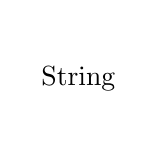
\begin{tikzpicture}[ 
	label distance=3mm,
	every label/.style={blue},
	event/.style={rectangle, draw, text centered,anchor=north},
	edge from parent/.style={very thick,draw=black!70,-latex},
	edge from parent path={(\tikzparentnode.south) -- ++(0,-0.50cm)-| (\tikzchildnode.north)},
	]
	\node [circle] (){String}
	
	;\end{tikzpicture}
	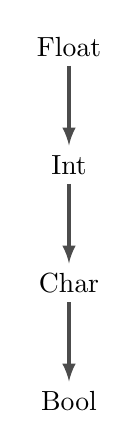
\begin{tikzpicture}
	[ 
	label distance=3mm,
	every label/.style={blue},
	event/.style={rectangle,draw,text centered,anchor=north},
	edge from parent/.style={very thick,draw=black!70,-latex},
	edge from parent path={(\tikzparentnode.south) -- ++(0,-0.50cm)-| (\tikzchildnode.north)},
	]
	\node []{Float}
	child {node {Int}
		child{ node {Char} 
			child { node {Bool}}
		}
	};
	\end{tikzpicture}
	\caption{Rappresentazione grafica della compatibilità tra tipi base.}
	\label{tab:albero}
\end{figure}


Oltre ai tipi di base  sono presenti due tipi composti: \texttt{*typ}, puntatore a \texttt{typ} e \texttt{Array[typ](dim)}, array di dimensione \texttt{dim} di elementi di tipo \texttt{typ}, dove \texttt{typ} è un tipo base o un tipo composto e \texttt{dim} è un intero; il tipo speciale \texttt{*Void} è utilizzato internamente per codificare il valore \texttt{Null}. È possibile assegnare il valore \texttt{Null} a qualsiasi elemento di tipo puntatore a \texttt{typ} qualunque sia il tipo \texttt{typ} puntato.
I tipi composti seguono le seguenti regole di compatibilità:
\begin{itemize}
\item un elemento di tipo \texttt{*typ1} è compatibile unicamente con elementi di tipo \texttt{*typ2}, un elemento di tipo \texttt{*typ1} è compatibile con un elemento di tipo \texttt{*typ2} se e solo se \texttt{typ1} è compatibile con \texttt{typ2} o se \texttt{typ1} = \texttt{Void};
\item un elemento di tipo \texttt{Array[typ1](dim1)} è compatibile unicamente con elementi di tipo \texttt{Array[typ2](dim2)}, un elemento di tipo \texttt{Array[typ1](dim1)} è compatibile con un elemento di tipo \texttt{Array[typ2](dim2)} se e solo \texttt{typ1} è compatibile con \texttt{typ2} e \texttt{dim1} = \texttt{dim2}.
\end{itemize}

Le regole di compatibilità tra tipi sono codificate all'interno della funzione \texttt{compatible} nel modulo \texttt{StaticAnalysis.hs}.
Sia \texttt{compatible typ1 typ2} equivalente a $typ_1 \leq typ_2$ nella notazione utilizzata in seguito, sia inoltre $\tau(exp)$ il tipo della espressione $exp$.
Le regole di derivazione per gli operatori unari sono riportare in tabella \ref{tab:unari}.

\begin{table}[]
\resizebox{\textwidth}{!}{
\begin{tabular}{l|l|l}
Operatore & Vincoli            & Tipo \\ \hline
$!exp$      & $\tau(exp) = Bool$ & $Bool$          \\
$-exp$      & $\tau(exp) \leq Float$   & \texttt{if} $\tau(exp) = Float$ \texttt{then} $Float$ \texttt{else} $Int$ \\
\end{tabular}
}
\caption{Regole di derivazione per gli operatori unari.}
\label{tab:unari}
\end{table}

Gli operatori binari sono classificati in \texttt{numerici}, \texttt{booleani}, \texttt{relazionali} come riportato in tabella \ref{tab:tipoOpBinari}. Le regole di derivazione per gli operatori binari sono definite in base alle possibili classi, tali regole sono riportate in tabella \ref{tab:binari}.

\begin{table}[]
\begin{tabular}{l|l}
Classe & Membri \\ \hline
Numerici & $\texttt{+},\ \texttt{-},\ \texttt{*},\ \texttt{/},\ \texttt{\^{}},\ \texttt{\%}$\\
Booleani & $\texttt{||},\ \texttt{\&\&}$ \\
Relazionali &$\texttt{<},\ \texttt{<=},\ \texttt{>},\ \texttt{>=} , \texttt{==},\ \texttt{!=} $ \\
\end{tabular}
\caption{Classificazione operatori binari.}
\label{tab:tipoOpBinari}
\end{table}

\begin{table}[]
\resizebox{\textwidth}{!}{
\begin{tabular}{l|l|l}
Operatore         &         Vincoli            & Tipo \\ \hline
$e_1\ op\ e_2$ t.c. $op \in Numerici$  &  $max(\tau(e_1), \tau(e_2)) \leq Float$ &  \texttt{if} $\tau(max(\tau(e_1), \tau(e_2))) = Float$ \texttt{then} $Float$ \texttt{else} $Int$ \\
$e_1\ op\ e_2$ t.c $op \in Booleani$ & $\tau(e_1) \leq Bool \wedge \tau(e_2) \leq Bool$ & $Bool$ \\
$e_1\ op\ e_2$ t.c. $op \in Relazionali$ & $\tau(e_1) \leq \tau(e_2) \wedge \tau(e_2) \leq \tau(e_1)$ & $Bool$\\
\end{tabular}
}
\caption{Regole di derivazione per gli operatori binari.}
\label{tab:binari}
\end{table}

Le regole di inferenza per le altre espressioni sono riportate in tabella \ref{tab:altro}.

\begin{table}[]
\resizebox{\textwidth}{!}{
\begin{tabular}{l|l|l}
Operatore         &         Vincoli            & Tipo \\ \hline
Array($e_1$, $\dots$, $e_n$) & $\forall_i (\tau(e_i) \leq max(\lbrace \tau(e_1), \dots, \tau(e_n)\rbrace)$ & $Array[max(\lbrace \tau(e_1), \dots, \tau(e_n)\rbrace)](n)$\\
if $e_c$ then $e_T$ else $e_F$ & $e_c \leq Bool \wedge e_T \leq max(\tau(e_T), \tau(e_F)) \wedge e_F \leq max(\tau(e_T), \tau(e_F))$ & $max(\tau(e_T), \tau(e_F))$\\
\end{tabular}
}

\caption{Regole di derivazione per l'operatore di creazione di array e l'operatore condizionale.}
\label{tab:altro}
\end{table}

Riguardo alle $L$-espressioni, ogni identificatore all'interno di un programma \texttt{Scala40} ha associato un tipo, nel caso delle variabili tale tipo è il tipo di dichiarazione della variabile, nel caso delle funzioni è il loro tipo di ritorno. Le regole di derivazione per gli operatori su $L$-espressioni di accesso ad un array, referenziamento e dereferenziamento sono riportate in tabella \ref{tab:LExp}.

\begin{table}[]
\resizebox{\textwidth}{!}{
\begin{tabular}{l|l|l}
Operatore         &         Vincoli            & Tipo \\ \hline
$*lexp$ & $\tau(lexp) = *typ$ dove $typ$ è un tipo qualsiasi & $typ$ \\
$\&lexp$ &                                                                                    & $*\tau(lexp)$\\
$lexp[e_a]$ & $\tau(e_a) \leq Bool \wedge \tau(lexp) = Array[typ](dim)$  con $typ$ e $dim$ qualsiasi & $typ$\\
\end{tabular}
}
\caption{Regole di derivazione per gli operatori su $L$-espressioni.}
\label{tab:LExp}
\end{table}

Negli statement di assegnamento è richiesto che il tipo della $R$-espressione sia compatibile con il tipo della $L$-espressione a cui si vuole assegnare.
Negli statement condizionali è richiesto che la condizione sia una espressione compatibile con il tipo $Bool$, se così non è viene lanciato un errore.

\subsection*{Vincoli riguardanti procedure e funzioni}
Alle procedure è assegnato come tipo di ritorno il tipo interno \texttt{Void}.
La signature della procedura principale di un programma \texttt{Scala40} è fissata a \texttt{main () : Void}, se si tenta di dichiarare una funzione/procedura con identificatore \texttt{main} e signature diversa da \texttt{main () : Void} viene riportato un errore.
Le chiamate di procedura non possono essere utilizzate come espressioni in quanto non hanno alcun valore di ritorno.

Riguardo al passaggio dei parametri attuali nelle chiamate di funzioni/procedure si richiede che il parametro attuale sia una $L$-espressione nel caso in cui il corrispondente parametro formale sia dichiarato con modalità per \texttt{riferimento}, per \texttt{risultato} o per \texttt{valore-risultato}. Nel caso in cui il parametro formale sia dichiarato con modalità per \texttt{valore} non ci sono vincoli sul corrispondente parametro attuale.
Si richiede una corrispondenza biunivoca tra la firma di una chiamata di procedura/funzione e la corrispondente firma di procedura/funzione, ogni parametro attuale oltre a rispettare i vincoli sulla modalità deve avere tipo compatibile con il tipo del corrispondente parametro formale.

Negli statement \texttt{return exp} si richiede che il tipo della espressione \texttt{exp} sia compatibile con il tipo dello scope in cui l'istruzione è contenuta, se così non è un errore viene lanciato.

Non è permesso utilizzare statement \texttt{return exp} all'interno di procedure, sono chiaramente permessi gli statement \texttt{return} senza espressione di ritorno; vale il viceversa nel caso delle funzioni.

\subsection*{Altri vincoli forti}
Gli statement \texttt{break} e \texttt{continue} sono utilizzabili solamente all'interno di cicli indeterminati (\texttt{while} e \texttt{do ... while}), nel caso ne si rilevi un utilizzo inappropriato viene lanciato un errore.

All'interno di un ciclo \texttt{for} la variabile di iterazione è considerata come una implicita dichiarazione locale del corpo.
\subsection*{Vincoli deboli}
La violazione dei seguenti vincoli non impedisce il proseguimento alle successive fasi della compilazione, tuttavia viene visualizzato un messaggio di avviso in quanto si ritiene che il comportamento ottenuto possa non essere quello cercato.

\begin{itemize}
	\item All'interno del blocco di codice di una funzione, deve essere presente almeno una istruzione $\texttt{return exp}$, con $\tau(exp)$ compatibile con il tipo di ritorno della funzione per ogni possibile percorso di esecuzione del blocco (per ogni valutazione delle guardie delle istruzioni $\texttt{if}$).
	\item Il programma deve contenere la dichiarazione di una procedura con firma $\texttt{main ()}$ al top level.
	\item Se una funzione viene chiamata senza assegnarne il valore di ritorno ad un'espressione.
\end{itemize}  
\section{Soluzioni non standard}
\subsection{Gestione del log tramite la monade Writer}
La gestione del log merita un discorso dedicato, per comprendere appieno cosa è stato svolto bisogna partire da una analisi del modulo \texttt{Errors.hs}.

Gli elementi di log, che possono essere \texttt{Warning} oppure \texttt{Errori}, contengono la posizione in cui si è verificata l'eccezione e la rispettiva eccezione.
Le eccezioni sono di tipo \texttt{TCException} e ogni eccezione ha un messaggio di notifica dedicato.

Il modulo \texttt{Environment.hs} che fornisce l'interfaccia al modulo di analisi statica per la gestione dell'environment del programma, utilizza una versione modificata della monade di default per la gestione degli errori utilizzata da BNFC. Nella versione da noi utilizzata in caso di errore viene ritornato un oggetto di tipo \texttt{TCException} invece che un oggetto \texttt{String}.

All'interno del modulo \texttt{StaticAnalysis.hs} è invece la monade \texttt{Writer} ad occuparsi di immagazzinare gli elementi di log creati durante l'analisi statica del programma.
La monade \texttt{Writer} si occupa di immagazzinare gli elementi di log all'interno di una lista di \texttt{LogElement}. Un nuovo elemento di log viene aggiunto alla lista tramite la funzione \texttt{tell}.

Giusto per chiarezza sintattica, nel nostro codice è stata aggiunta una funzione \texttt{saveLog} che è poco più che un alias della funzione \texttt{tell}, ed è stato definito l'alias \texttt{Logger a} per \texttt{Writer [LogElement] a}.
Ogni funzione del modulo di analisi statica che può scovare un'eccezione durante l'analisi dell'albero di sintassi astratta, ritorna dunque un elemento \texttt{Logger a}.

\subsection{Gestione delle istruzioni TAC tramite la monade State}

Per la gestione della creazione delle istruzioni TAC durante la creazione di quest'ultimo, è stata utilizzata la monade {\tt State a}. Questa permette di manipolare l'inserimento di nuove istruzioni, la creazione di nuove etichette e di nuovi temporanei, in modo equiparabile ad un cambio di stato in una computazione. La creazione e l'inserimento di una nuova istruzione nel codice TAC corrispongono, appunto, ad una modifica dello stato corrente, La monade {\tt State a} utilizza due funzioni per operare su quest'ultimo: {\tt get}, per ottenere lo stato, e {\tt put} per aggiornarlo. 

La monade {\tt State a} utilizzata durante la creazione del Three Address Code opera su stati formati da tuple di quattro elementi:
\begin{itemize}
    \item un intero che indica l'indice dell'ultimo temporaneo creato;
    \item un intero che indica l'ultima etichetta creata;
    \item la lista di istruzioni TAC che compongono il TAC in output;
    \item una lista di liste di istruzioni TAC. Ogni lista contiene un insieme di istruzioni di una singola funzione. 
\end{itemize}

Lo stato viene modificato nel momento in cui: si crea una nuova etichetta e/o un nuovo temporaneo tramite le funzioni {\tt newLabel} e {\tt newTemp}, rispettivamente (per evitare duplicazioni tra le istruzioni) e quando una nuova istruzione TAC di una funzione viene inserita nella lista delle istruzioni di quella funzione (tramite la funzione {\tt out}). Inoltre, vi è una modifica dello stato nel momento in cui tutti gli statetement di una funzione sono stati tradotti in istruzione TAC: l'insieme delle istruzioni di quella funzione vengono aggiunte in testa all'insieme delle istruzioni TAC principale (quelle che compongono il TAC in output), tramite la funzione {\tt pushCurrentStream}.

Nel file {\tt ThreeAddressCode.hs} è stato utilizzato {\tt TacState a} come alias per {\tt State (Int, Int, [TAC], [[TAC]]) a}, dove {\tt TAC} è un'istruzione TAC.
\section{Descrizione soluzione}

\subsection{Il modulo di analisi statica}
In questa sezione viene fornita una breve descrizione della logica retrostante il funzionamento del modulo di analisi statica \texttt{StaticAnalysis.hs}.

Il modulo di analisi statica fornisce un'interfaccia alle restanti componenti del compilatore, che permette di ottenere un albero di sintassi astratta annotato ed eventualmente una lista di log a partire da un programma \texttt{Scala40} rappresentato in sintassi astratta.

Per la gestione dei log si rimanda alla sezione riguardante le tecniche non standard utilizzate.

Il modulo è stato progettato seguendo un approccio \textit{top-down}, andando di volta in volta a risolvere i sotto-problemi che ci apparivano dinanzi.

Il modulo di analisi statica fa largo uso del modulo \textit{Environment.hs} che gli offre un'interfaccia per la gestione dell'environment del programma sotto analisi. 

L'environment di un programma è una pila di \textit{scope}, dove ogni scope è formato da: una \textit{tabella di lookup} che mette in corrispondenza gli identificatori definiti all'interno dello scope con le informazioni a riguardo, un \textit{tipo} che eredita dalla funzione in cui lo scope è stato creato ed infine un \textit{valore booleano} che indica se nello scope è presente o meno  un \texttt{return} con tipo compatibile con quello dello scope.

Il modulo \texttt{Environment.hs} fornisce tutte le funzioni necessarie per la gestione dell'environment di un programma. La funzione \texttt{lookup}  permette di ottenere le informazioni a riguardo di un identificatore dichiarato in precedenza nello scope corrente, o in un \textit{super-scope} nel quale lo scope corrente è contenuto; nel caso in cui l'identificatore cercato non sia trovato un eccezione viene ritornata.
La funzione \texttt{update} permette di inserire una nuova corrispondenza \textit{identificatore-info} nello scope corrente, nel caso in cui l'identificatore che si sta cercando di inserire fosse già stato dichiarato in precedenza all'interno dello scope corrente una eccezione viene ritornata.
Per ottenere il tipo dello scope corrente è presente la funzione \textit{getScopeType}, la funzione \textit{hasReturn} ritorna invece il valore booleano che indica se nello scope corrente è presente o meno un \texttt{return} di tipo coerente con quello dello scope; quando un tale \texttt{return} viene trovato la funzione \texttt{setReturnFound} permette di impostare tale valore booleano a \texttt{True}.
La funzione \texttt{addScope} permette di aggiungere un nuovo scope all'environment, la funzione prende come argomento il tipo dello scope che si vuole aggiungere. Qui è importante porsi una domanda:
\begin{center}
Quale tipo viene passato ad \texttt{addScope}?
\end{center}
La risposta è: \textit{dipende}. 
Se lo scope è lo scope globale del programma per una nostra convenzione esso ha tipo \texttt{TSimple\_TypeVoid}; se lo scope viene creato da una dichiarazione di funzione, allora il tipo passato ad \texttt{addScope} è quello della funzione dichiarata; infine se lo scope viene aggiunto dalla creazione di un blocco di statements, allora il tipo passato ad \texttt{addScope} è quello dello scope in cui il blocco di statements è racchiuso.
Non è difficile vedere che tali accorgimenti verificano la proprietà stabilità per il tipo di uno scope, ossia che il tipo di uno scope coincide con il tipo della funzione in cui è racchiuso.

Forniamo ora una breve panoramica del funzionamento del modulo di analisi statica \texttt{StaticAnalysis.hs}. La funzione principale del modulo è \texttt{typeCheck} che preso un programma rappresentato in sintassi astratta di \texttt{Scala40} ritorna tale programma annotato ed eventualmente una lista di log.
Il compito di annotare gli elementi della sintassi astratta e di aggiungere eventuali log alla lista di log ogni qual volta venga rilevata una eccezione è affidato alle funzioni \texttt{infer*} (per esempio: \texttt{inferDecl}, \texttt{inferStm}, \texttt{inferExp}, etc.), tali funzioni preso un elemento della sintassi astratta effettuano i controlli per verificare che tale elemento sia coerente con le specifiche del linguaggio \texttt{Scala40} e nel caso non lo siano tramite la funzione \texttt{saveLog} si occupano di aggiornare la lista di log; al termine dei controlli l'elemento analizzato viene ritornato arricchito con annotazioni quali le informazioni sugli identificatori utilizzati e il tipo delle espressioni coinvolte. 

Le funzioni \texttt{infer*} hanno tutte un comportamento naturalmente ricorsivo, si prenda per esempio il caso di una dichiarazione di variabile con assegnamento di un valore, per poter inferire la dichiarazione e determinare se è valida o meno è necessario inferire l'espressione che si sta cercando di assegnare alla variabile e verificare che i tipi combacino.

Per una nostra decisione personale, nel caso in cui si stia inferendo un elemento che coinvolge una espressione la quale abbiamo già verificato essere problematica, non vengono aggiunte al log nuove eccezioni riguardanti l'elemento sotto-analisi. Questa scelta è giustificata dal desiderio di eliminare ridondanza negli errori, dato che una espressione errata, potrebbe portare ad una lunga serie di errori a catena in tutti gli elementi in cui è compresa.

Per ottenere questo comportamento, abbiamo nella sintassi astratta un tipo interno \texttt{SType\_Error} che viene assegnato alle espressioni che generano un'eccezione, o alle espressioni le cui sotto-espressioni generano eccezioni. Se un qualsiasi elemento ha come sotto-espressione una espressione di tipo \texttt{SType\_Error} non vengono generate ulteriori eccezioni riguardo all'interazione di tale sotto-espressione con l'elemento considerato.

Le annotazioni aggiunte dal modulo di analisi statica riguardano esclusivamente le espressioni, sia R-espressioni (elementi \texttt{Exp}), sia L-espressioni (elementi \texttt{LExp}. Le espressioni annotate sono identificate rispettivamente dagli elementi di sintassi astratta interni: \texttt{ETyped} per le R-espressioni e da \texttt{LExpTyped} per le L-espressioni. Entrambi gli elementi condividono la stessa struttura, una espressione tipata contiene la espressione, il suo tipo, e la locazione in cui viene utilizzata. Un ulteriore caratteristica delle espressioni tipate è che la locazione contenuta all'interno di un identificatore utilizzato all'interno dell'espressione non è la locazione di utilizzo, che invece è in un campo apposito, ma è la locazione di dichiarazione dell'identificatore.
La locazione di dichiarazione di un identificatore utilizzato all'interno di una espressione ci risulta fondamentale per la successiva fase di sgenerazione del codice TAC.
La definizione degli elementi tipati con le loro proprietà è presente all'interno del modulo \texttt{Typed.hs}.




\subsection{Descrizione soluzione - Three Address Code}

Il Three Address Code (TAC) viene costruito a partire dall'albero annotato risultante dall'analisi di semantica statica. Per la costruzione viene fatto largo uso della monade State, descritta nella sezione precedente.

Gli indirizzi utilizzati per le istruzioni del TAC sono dei seguenti tipi:
\begin{itemize}
    \item Letterali: per valori costanti di tipo base.
    \item Indirizzi di variabile e di funzioni: hanno la seguente forma:
    \begin{center}
        {\tt ident@loc}
    \end{center}
    dove {\tt ident} è il loro identificatore e {\tt loc} la locazione di dichiarazione.
    \item Temporanei: utilizzati per identificare espressioni.
\end{itemize}
Inoltre, nel TAC sono presenti le etichette che vengono utilizzate per indicare una locazione univoca nel flusso di esecuzione. Nel caso delle funzioni, come etichetta, viene utilizzato il loro indirizzo.
%%%%%%%%%%%%%%%%%%%%%%%%%%%%%%%%%%%%%% genProg, genDecls, genDecl

La costruzione del Three Address Code inizia dalla funzione {\tt genProg} che ha i seguenti compiti:
\begin{itemize}
    \item Inserire un'etichetta in fondo a tutte le istruzioni (e il relativo {\tt Call} dopo le dichiarazioni globali) se durante l'analisi di semantica statica non è stato trovato una funzione main da cui far partire la computazione. In alternativa, viene inserita un'istruzione {\tt Goto} all'etichetta del main;
    \item iniziare la discesa nell'albero annotato per poter costruire le singole istruzioni, tramite la funzione {\tt genDecls}.
\end{itemize}

La funzione {\tt genDecls} prende in input una lista di dichiarazioni e le scorre producendo le relative istruzioni TAC. Questo avviene tramite la funzione {\tt genDecl}; questa divide le dichiarazioni nei quattro casi possibili:
\begin{itemize}
    \item Dichiarazione di variabile con assegnamento: viene creato un nuovo indirizzo a partire dall'identificatore della variabile e dalla sua locazione di dichiarazione. Gli viene assegnato un valore tramite la funzione {\tt genExpAddr} che permette di evitare la creazione di temporanei inutili quando ci troviamo nel caso di un'espressione semplice (es. $x = 3$, $*y= x$, $x = y + z$ ecc.) ed esegue i necessari cast.
    \item Dichiarazione di variabile: come nel caso precente costruiamo un indirizzo a partire da identificatore e locazione, e gli assegnamo un valore di default (\label{table:valori_default}) tramite la funzione {\tt buildDefaultValue}.
    \item Dichiarazione di funzione/procedura: in questo caso viene creata una nuova etichetta per la funzione. Viene chiamata la funzione {\tt genBlock} che (tramite {\tt genStms}) controlla la presenta dell'istruzione {\tt return} (nel caso delle procedure verrà aggiunto un'istruzione di return vuoto) e costruisce tutte le istruzioni TAC relative al corpo della funzione. Al termine di questo processo le istruzioni TAC che sono state create vengono estratte tramite operazione di pop dalla lista di liste di istruzioni dello stato e inserite in testa al codice globale del TAC. Questo viene fatto per far sì che una funzione dichiarata nel corpo di un'altra venga, inserita sopra quest'ultima a livello di Three Address Code, e non al suo interno. 
    
    Inoltre, se la dichiarazione si trova nello scope globale e l'identificatore utilizzato è $\texttt{main}$, viene controllato che la funzione abbia una firma specifica: {\tt def main()}.
\end{itemize}

\begin{table}
\centering
    \begin{tabular}{|c c|} 
        \hline
        Tipo & Valore di default \\ [0.5ex] 
        \hline\hline
        Int & 0 \\ 
        Float & 0.0  \\
        Char & \textbackslash0 \\
        String &  "" \\
        Bool & False \\ 
        Pointer & Null\\
        Array & - \\[1ex] 
        \hline
    \end{tabular}
    \caption{Valori di default}
    \label{table:valori_default}
\end{table}


%%%%%%%%%%%%%%%%%%%%%%%%%%%%%%%%%%%%%% genBlock, genStms, genStm

Ogni funzione è costituita da un insieme di statement (contenuti in un blocco). La funzione che si occupa di percorrere tutti gli statement di un blocco è {\tt genStms}, che restituisce {\tt True} se l'ultimo statement è un {\tt return} (per evitare che nel TAC compaiano due istruzioni {\tt return} consecutive). Nel contempo vengono esaminati gli statement singolarmente tramite la funzione {\tt genStm}.
Quest'ultima prende in esame tutti i possibili statement:
\begin{itemize}
    \item Dichiarazione: viene riutilizzata {\tt genDecl} per la gestione delle dichiarazioni interne al blocco.
    \item Blocchi interni: viene riutilizzata la funzione {\tt genBlock}.
    \item Assegnamenti: un assegnamento ha la seguente forma:
    \begin{center}
        {\tt Lexpression = RExpression}
    \end{center}
    Le {\tt l-expression} comprendono: accessi ad array, variabili puntatori e identificatori di variabile. La loro gestione avviene tramite la funzione {\tt genLexp}. Le {\tt r-expression} oltre che le {\tt LExpression}, comprendono le espressioni.
    \item Chiamata di procedura: vengono create le istruzioni che indicano i parametri passati alla funzione (tramite la funzione {\tt genParams} che crea istruzioni {\tt Param addr}) e viene creata un'istruzione {\tt Call} del TAC. La funzione {\tt genParams} si occupa anche di deferenziare la variabile passata alla funzione se il metodo di passaggio richiesto è {\tt ref}, {\tt res}, {\tt valres}. Al momento della stampa, le funzione già definite nel linguaggio (es. {\tt writeInt}) avranno, al posto della locazione specificata nell'indirizzo, la parola {\tt default} (es. {\tt writeInt@default}).
    \item Return: se l'istruzione {\tt return } ritorna un'espressione essa viene gestita tramite {\tt genExpAddr}, che in caso di espressioni complesse (non binaria tra due identificatori o unaria) restituisce un temporaneo.
    \item Break e Continue: viene creata un'istruzione {\tt Goto} con associata un'etichetta che indica l'inizio del ciclo in caso di {\tt continue} e l'istuzione subito dopo il ciclo nel caso di {\tt break}.
    
    \item For: oltre che all'istruzione di controllo per le varie iterazioni, viene inserito in coda a tutte le istruzioni TAC relative al corpo del ciclo, l'istruzione di incremento dell'iteratore. 
    
    \item Do-While: viene modificato lo stato con le etichette relative ai {\tt break} e {\tt continue}. In questo caso le etichette create sono tre: quella relativa all'inizio del ciclo (utilizzata dalla condizione di iterazione), quella che indica la posizione del controllo dell'iterazione (utile per il {\tt Goto}  del {\tt continue}) e quella che indica l'istruzione successiva alla posizione di controllo (utile per il {\tt Goto} del {\tt break}). Al termine delle istruzioni relative al ciclo, il valore dello stato relativo alle etichette {\tt break} e {\tt continue} viene ristabilito al precedente valore;
    \item While: come nel caso precedente vengono create le etichette per il {\tt break} e il {\tt continue}, che, vengono gestite come nel caso precedente. In questo caso le etichette create sono solo due: quella che rimanda all'inzio del ciclo e quella che rimanda alla prima istruzione dopo il ciclo;
    \item If: banalmente vengono create le istruzioni relative agli statement relativi all'{\tt if} e all'{\tt else}. Se il corpo dell'{\tt else} è vuoto, allora l'etichetta {\tt labelElse} dopo le istruzioni del caso {\tt if} non viene generata.
\end{itemize}

Sia per quanto riguarda gli {\tt If} e i cicli ({\tt For, Do-While} e {\tt While}) la gestione delle etichette avviene tramite la funzione {\tt genCondition}, che, presa l'espressione della condizione e le due etichette che indicano dove spostarsi in caso essa sia vera o meno, gestitisce la creazione dei {\tt Goto} ed esegue il controllo del flusso. La funzione {\tt genCondition} viene utilizzata in particolar modo per evitare controlli superflui (es. nella condizione {\tt a \&\& b} se {\tt a} è falsa, non serve valutare anche {\tt b} e il controllo può passare all'etichetta relativa al caso {\tt False} della condizione).

%%%%%%%%%%%%%%%%%%%%%%%%%%%%%%%%%%%%%% genExp

La generazione delle istruzioni riguardanti le espressioni viene gestita tramite la funzione {\tt genExpAddr} che restituisce l'indirizzo TAC dell'espressione: un letterale nel caso di espressioni composte da un solo letterale o un nuovo temporaneo nel caso di dereferenziazioni, LExpression, accessi ad array o espressioni simili a quelle descritte nel caso dell'assegnamento. Se il tipo dell'espressione tipata restituita durante la fase di analisi statica è diverso (ma sicuramente compatibile) con quello della sottoespressione che si sta analizzando, allora viene eseguito un {\tt cast} implicito.

%%%%%%%%%%%%%%%%%%%%%%%%%%%%%%%%%%%%%% Conslusione

Terminate tutte le dichiarazioni presenti nello scope globale, vengono inserite in testa alla lista di istruzioni TAC tutte le dichiarazioni di variabili globali seguite dall'istruzione {\tt Goto} alla funzione {\tt main} se presente, oppure all'etichetta {\tt l0} in fondo a tutte le istruzioni (evitando così che tutte le altre funzioni vengano eseguite sequenzialmente).

La stampa ordinata delle istruzioni TAC avviene tramite le funzioni in {\tt PrintTAC.hs}. Per aumentare la leggibilità del codice TAC sono stati aggiunti numerosi commenti, ad esempio quelli relativi all'inizio e fine di una funzione o dei cicli. Relativamente ai commenti, al fianco delle operazioni di addizione, sottrazione, moltiplicazione, divisione, modulo è stato aggiunto un commento con il nome preciso dell'istruzione che sta venendo eseguita, ad esempio {\tt MulInt} per la moltiplicazione tra interi o {\tt PlusFloat} per la somma di float. Ciò è stato fatto per aumentare la comprensibilità delle espressioni, che altrimenti, con i soli simboli {\tt +}, {\tt -}, {\tt *}, {\tt /}, {\tt \%}, sarebbero risultate essere indistiguibili nei due casi (Float e Int)




\end{document}